\chapter{converter}
%--------------------------------------------------------------------------------
\section{Informations on the formats handled}
%--------------------------------------------------------------------------------

%--------------------------------------------------------------------------------
\subsection{SERAFIN format}
%--------------------------------------------------------------------------------

The SERAFIN format was created for \telemacsystem by EDF. It consists of a binary file
containing the mesh information and the results.  The boundary conditions are
written in an ASCII file or defined in a user's function in \telemacsystem.  What the
file contains is described in the following:

\begin{itemize}
\setlength{\itemsep}{1pt}
\setlength{\parskip}{0pt}
\setlength{\parsep}{0pt}
\item title
\item i,j: number of variables (linear discretization and quadratic
discretization)
\item i+j records of 'name and units of variable' the 16 first characters are
the name and the last 16 are the unit
\item 10 integers: the $7^{th}$ integer gives the number of layers, the
$10^{th}$ indicates that the date is present
\item 4 integers: number of elements (\textit{nelem}), number of points
(\textit{npoin}), number of points defining an element (\textit{ndp}), 1
\item ikles(\textit{npoin}*\textit{ndp}): table of connectivity elements $->$
points
\item ipobo(\textit{npoin}): assigns 1 if the node is a boundary node, 0
otherwise.  If the mesh is distributed ipobo is replaced by
knolg(\textit{npoin}) the local-to-global numbering table
\item x(\textit{npoin}): x coordinates
\item y(\textit{npoin}): y coordinates
\item loop for each time step
\begin{itemize}
\setlength{\itemsep}{1pt}
\setlength{\parskip}{0pt}
\setlength{\parsep}{0pt}
\item The time T (real)
\item loop for each variable \textit{var}
\begin{itemize}
\setlength{\itemsep}{1pt}
\setlength{\parskip}{0pt}
\setlength{\parsep}{0pt}
\item array of \textit{npoin} containing the results for the variable
\textit{var} at time T
\end{itemize}
\item End of the loop on the variables
\end{itemize}
\item End of the loop on the time steps
\end{itemize}

The number of layers is used for \telemac{3} meshes, which is built by extruding the
2D horizontal mesh.  In 3D the z coordinate is the first variable.

The SERAFIN format is used by most of the codes of the \telemacsystem. It can be read
by TECPLOT with the use of a plugin.  The mesh generators Rubens, BlueKenue
and Fudaa PrePro can generate meshes in SERAFIN format.

The pre-\&post-processing tools for parallel simulations, namely
\verb+partel/gretel+, support the SERAFIN format.

Reals are defined in single precision in the SERAFIN format. An identical format
called \textbf{SELAFIND} contains reals in double precision.

%--------------------------------------------------------------------------------
\subsection{MED format}
%--------------------------------------------------------------------------------

The MED3.0.4 format is SALOME's native format. Each MED file is binary.
Information are accessed through the functions of the MED library.

This library is divided in the following sections:

\begin{tabular}{p{70pt}@{ : }p{200pt}p{50pt}}
  \textbf{Library} & Get library informations & mlb* \\
  \textbf{File} & Open/close file & mfi* \\
  \textbf{Profile} & Build selection of nodes & mpf*\\
  \textbf{Mesh} & Information about the mesh (dimension, name, type, coordinates, elements connectivity, \ldots) & mmh*\\
  \textbf{Family} & Read/write of families & mfa*\\
  \textbf{Equivalence} & Link between elements & meq*\\
  \textbf{Joint} & Build a link between two nodes/elements from different partitions (Used for distributed mesh)& msd*\\
  \textbf{Structure} & Creation of new elements & mse*\\
  \textbf{element} & & \\
  \textbf{Field} & Read/write results information & mfd*\\
  \textbf{Link} & Handle link between two meshes & mln*\\
  \textbf{Localization} & Handle element referencing & mlc*\\
  \textbf{Interpolation} & Handle interpolation functions & mip*\\
  \textbf{Parameter} & Read/write constants & mpr*\\
  \textbf{Filter} & Build sub-domains of elements & mfr*\\
\end{tabular}

The library is written mainly in C/C++ but has a Fortran 90 wrapper.
The MED format is used in the \telemacsystem. It can be visualized or modified in SALOME.

%--------------------------------------------------------------------------------
\subsection{UNV format}
%--------------------------------------------------------------------------------

UNV files are ASCII. They are made of a list of sections.

Here is the description of a section:

\begin{itemize}
\setlength{\itemsep}{1pt}
\setlength{\parskip}{0pt}
\setlength{\parsep}{0pt}
\item -1
\item section number
\item \ldots section information \ldots
\item -1
\end{itemize}
In the program we consider 3 sections:
\begin{itemize}
\setlength{\itemsep}{1pt}
\setlength{\parskip}{0pt}
\setlength{\parsep}{0pt}
\item The title section containing the title.
\item The coordinate section containing the coordinates and the color of each
node.
\item The connectivity section containing the connectivity table for the
elements and the color of each element.
\end{itemize}

A complementary ASCII file containing the number of nodes and the total number
of elements also exists (in 3D we can have both 3D and 2D elements).

Note that the UNV format is only used in \estel within the \telemacsystem.
More information about families are also available but they are not used in
\estel.
Most mesh generators can generate meshes in UNV format.
SALOME can read a mesh in UNV format.

%--------------------------------------------------------------------------------
\subsection{VTK format}
%--------------------------------------------------------------------------------

The legacy VTK file format consists of five basic parts:

\begin{enumerate}
\setlength{\itemsep}{1pt}
\setlength{\parskip}{0pt}
\setlength{\parsep}{0pt}
\item The first part is the file version and identifier. This part contains the
single line: \verb+# vtk DataFile Version x.x+.  This line must be exactly as
shown with the exception of the version number x.x, which will change with
different releases of VTK. (Note: the current version number is 3.0. Version
1.0 and 2.0 files are compatible with version 3.0 files).
\item The second part is the header. The header consists of a character string
terminated by the end-of-line character \verb+\n+. The header contains 256
characters at most. It can be used to describe the data and include any other
pertinent information.
\item The third part is the file format. The file format describes the type of
file, either ASCII or binary.  On this line the word 'ASCII' or 'BINARY' has to
be present.
\item The fourth part is the dataset structure. The geometry part describes the
geometry and the topology of the dataset. This part begins with a line
containing the keyword DATASET followed by a keyword describing the type of
dataset.  Then, depending upon the type of dataset, other keyword/data
combinations define the actual data.
\item The final part describes the dataset attributes. This part begins with
the keywords POINT\_DATA or CELL\_DATA, followed by an integer number
specifying the number of points or cells, respectively. (There is no constraint
on the order of appearance of POINT\_DATA or CELL\_DATA). Other keyword/data
combinations then define the actual dataset attribute values i.e., scalars,
vectors, tensors, normals, texture coordinates, or field data.
\end{enumerate}

%--------------------------------------------------------------------------------
\subsection{CGNS format}
%--------------------------------------------------------------------------------

CGNS (CFD General Notation System, latest version 3.1.3) originated in 1994 as
a joint effort between Boeing and NASA, and has since grown to include many
other contributing organizations worldwide. It is an effort to standardize CFD
input and output, including grid (both structured and unstructured), flow
solution, connectivity, boundary conditions, and auxiliary information. CGNS
is also easily extensible, and allows for file-stamping and
user-inserted-commenting. It employs ADF (Advanced Data Format) and/or HDF5
(Hierarchical Data Format) as a database manager which creates binary files
that are portable across computer platforms. It provides a layer of software,
the CGIO Interface which allows access to these database managers at a
low-level, and a second layer of software known as the Mid-Level Library, or
API (Application Programming Interface), which eases the implementation of
CGNS into existing CFD codes.

A CGNS file is an entity that is organized (inside the file itself) into a set
of "nodes" in a tree-like structure, in much the same way as directories are
organized in the UNIX environment.  Strictly speaking, because links may be
used to store information in multiple files, there is no notion of a CGNS
file, only of a CGNS database implemented within one or more files.  However,
throughout this document the two phrases are used interchangeably. The top-most
node is referred to as the "root node." Each node below the root node is
defined by both a name and a label, and may or may not contain information or
data. Each node can also be a "parent" to one or more "child" nodes.  A node
can also have as a child node a link to a node elsewhere in the file or to a
node in a separate CGNS file altogether. Links are transparent to the user:
the user "sees" linked children nodes as if they truly exist in the current
tree. An example of a CGNS tree-like structure is shown below.

\begin{figure} [ht]
\centering
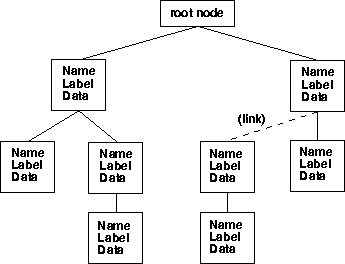
\includegraphics[scale=0.5]{graphics/cgns.png}
\caption{Example CGNS tree-like structure.}
\end{figure}

%--------------------------------------------------------------------------------
\section{\label{upgrades}Description of the new features}
%--------------------------------------------------------------------------------

All the upgrades were included in \stbtel using new parameters, added to the
dictionary. The program still uses the steering file. A parameter determines
whether the new features or the old ones are used.  First are described the new
parameters and features, then will be describe the issues encountered and the
answers given for each format.

%--------------------------------------------------------------------------------
\subsection{Modifications in \stbtel's main program}
%--------------------------------------------------------------------------------

The following table describes the new parameters available for the steering
file:\\

\begin{tabular}{p{140pt}@{ : }p{200pt}}
\textbf{CONVERTER} & (Boolean) If true then use the new features.\\
\textbf{DEBUG} & (Boolean) If true display debug informations.\\
\textbf{SELAFIN IN DOUBLE PRECISION} & (Boolean) If true the SERAFIN file will be read/written in double precision.\\
\textbf{INPUT FILE FORMAT} & (String) The format of the input file, MED, UNV, SERAFIN.\\
\textbf{OUTPUT FILE FORMAT} & (String) The format of the output file, MED, UNV, SERAFIN, VTK.\\
\textbf{INPUT FILE} & (String) The name of the input file.\\
\textbf{BOUNDARY FILE} & (String) The name of the boundary file if it exists (optional).\\
\textbf{LOG FILE} & (String) The name of the complementary file, for the UNV format only.\\
\textbf{OUTPUT FILE} & (String) The name of the output file.\\
\textbf{OUTPUT BOUNDARY FILE} & (String) The name of the output boundary file if it exists (optional).\\
\textbf{OUTPUT LOG FILE} & (String) The name of the output complementary file, for the UNV format only.\\
\end{tabular}

The program works in two steps:
\begin{itemize}
\setlength{\itemsep}{1pt}
\setlength{\parskip}{0pt}
\setlength{\parsep}{0pt}
\item First the file is read and the mesh object structure is filled in.
\item The information from the mesh object structure are written into the
output file.
\end{itemize}

All the format's functions (read/write) are contained in the file
\verb+conv_+\textit{format}\verb+.f+ (where \textit{format} stands for SERAFIN,
MED, \ldots).\\

The table below shows which conversions are possible:

\begin{center}
\begin{tabular}{|l||*{5}{c|}}
\hline
\diagbox{Input}{Output}  & SERAFIN    & MED      & UNV      & CGNS     & VTK    \\
\hline
\hline
SERAFIN     & X         & \checkmark & \checkmark & \checkmark & \checkmark \\
\hline
MED     & \checkmark & X        & \checkmark & \checkmark & \checkmark \\
\hline
UNV     & \checkmark & \checkmark & X        & \checkmark & \checkmark \\
\hline
CGNS    & \checkmark & \checkmark & \checkmark & X        & \checkmark \\
\hline
\end{tabular}\\
\checkmark : Available, X : Unauthorized
\end{center}

The UNV format is the only format that can not manage results. It only
contains the mesh and the colors.

\stbtel handles distributed meshes only for MED and SERAFIN format.

Some formats use a file for each time step for the results file, this is the
case for the VTK format.

Instead of running \stbtel with a steering a script, named \verb+covnerter.py+,
has been created in order to launch the converter in a one-line-command. This
script is written in \textbf{Python 2.6}.

Here is the way it works (To see to following message run \verb+converter.py --help+):
\begin{verbatim}
Usage: converter.py input-file-name -o output-file-name [options]
Example: converter.py coarse.slf -b coarse.cli -o coarse.med --debug
Where coarse.slf is the mesh in SERAFIN fornat,
      coarse.cli is the boundary conditions file and
      coarse.med the converted mesh in MED format.

Options:
  -h, --help            show this help message and exit
  -o OUTPUTFILE, --output-file=OUTPUTFILE
                        name of the output file also defines the
                        output format
  --input-format=INPUTFORMAT
                        name of the input format, overwrites
                         input detected byextension
  --output-format=OUTPUTFORMAT
                        name of the output format, overwrites
                        output detectedby extension
  --output-boundary-file=OUTBOUNDARYFILE
                        name of the output boundary file
  -b BOUNDARYFILE, --boundary-file=BOUNDARYFILE
                        name of the boundary file
  -l LOGFILE, --log-file=LOGFILE
                        name of the log file
  -n NDOMAINS, --ndomains=NDOMAINS
                        number of sub-domains of the distributed mesh
  --srf-bnd             tell stbtel to read the boundary conidtion
                        from theboundary file
  -s, --silent          disable stbtel output informations
  --debug               Enable debug mode which displays more
                        informationsduring run time
  --dx=DX               Value to add to the X coordinates
  --dy=DY               Value to add to the y coordinates
  -r ROOTDIR, --rootdir=ROOTDIR
                        specify the root, default is taken
                        from config file
\end{verbatim}

The conversion of all the files of a distributed mesh in one run is only
available in the python script.

%--------------------------------------------------------------------------------
\subsection{The mesh object structure}
%--------------------------------------------------------------------------------

Here is a description of the object's structure that is used by the converter.
This object makes it easier to add new formats, for each format only two
functions will be needed one to fill the mesh object by reading the file and
one writing the file using the mesh object's data.  A similar object is used in
the \bief library to store mesh information.  This object is used as a common
ground between all the formats handled by the converter.

\begin{description}
\setlength{\itemsep}{1pt}
\setlength{\parskip}{0pt}
\setlength{\parsep}{0pt}
\item[Common Block]
\item[title] Name of the mesh.
\item[description] Description of the mesh (only MED).
\item[ndim] Dimension of the domain (2 or 3).
\item[nelem] Number of elements.
\item[npoin] Number of nodes.
\item[ndp] Number of points per element.
\item[type\_elem] Type of element (triangle, quadrilateral, tetrahedron, prism).
\item[nptfr] Number of boundary nodes.
\item[ib] Table of 10 integers: ib(10) (only used for SERAFIN).
\item[ikles] Connectivity table: ikles(nelem*ndp).
\item[ipobo] Flag for boundary node: ipobo(npoin).
\item[x] x coordinates: x(npoin).
\item[y] y coordinates: y(npoin).
\item[z] z coordinates: z(npoin).
\item[namecoo] Name of the coordinates: namecoo(ndim).
\item[unitcoo] Unit of the coordinates: unitcoo(ndim).
\item[knolg] Global number of point: knolg(npoin).
\item[Results information]
\item[nvar] Total number of variables.
\item[namevar] Name of the variables: namevar(maxvar).
\item[unitvar] Unit of the variables: unitvar(maxvar).
\item[timestep] Number of time steps.
\item[times] Table containing for each time step its value in seconds: times(timestep).
\item[res] Results for all the time steps and all the variables: res(timestep,nvar,npoin).
\item[Families information]
\item[nfam] Number of families.
\item[idfam] id of the family: idfam(nfam).
\item[valfam] Value of each family: valfam(nfam).
\item[namefam] Name of each family: namefam(nfam).
\item[ngroupfam] Number of group of each family: ngroupfam(nfam).
\item[groupfam] Group of each families: groupfam(nfam,10).
\item[Boundary information]
\item[nbor] Local number of each boundary node: nbor(nptfr).
\item[libor] Value of each boundary node: libor(nptfr).
\item[\estel second element type information]
\item[nelem2] Number of elements.
\item[ndp2] Number of points per element.
\item[type\_elem2] Type of element.
\item[ikles2] Connectivity table: ikles2(nelem*ndp).
\item[Color information]
\item[color] Color of a node: color(npoin).
\item[ncolor] Color of an element: ncolor(nelem).
\item[ncolor2] Color of an element (\estel's second element): ncolor2(nelem2).
\end{description}


%--------------------------------------------------------------------------------
\subsection{SERAFIN}
%--------------------------------------------------------------------------------

The code is implemented following the \bief library standards as much as
possible. Three subroutines are used to read the mesh information
\verb+readgeo1+, \verb+readgeo2+, \verb+readgeo3+. But they do not read the
title, the variable information nor the result information. The functions
\verb+lit/ecri2+ of the \bief are used to read and write the extra information.
The \verb+readgeo+ functions contain an optional parameter in order to handle
double precision real.  But in Fortran for the optional parameter to work, a
function has to be declared in an interface and the function in which it is
called must contain the line \verb+use module+ which calls the interface.

When the results part of the SERAFIN file is reached, the results table
(\textbf{res} in mesh object) cannot be allocated because the number of time
steps is unknown at this stage.  To compute this value a quick read trough the
rest of the file is carried out in order to count the number of records.  The
file is then rewound, the results table can now be allocated and filled in.

Because the function rewind causes problems with some machines/compilers (for
instance with GCC-4.1.2) the file is closed and re-opened instead.

An extra file which contains the read/write functions for the boundary file has
been added.

Note that the title is set to have a length of 72 characters in the \bief
library but it is defined with a length of 80 in the TECPLOT plug-in and the
\verb+sel2vtk+ program.

%--------------------------------------------------------------------------------
\subsection{MED}
%--------------------------------------------------------------------------------

Families are used to assign a value to a point. They can also be used to
represent colors or boundary conditions.  A family and a group is created for
each value (\verb?lihbor*100+liubor*10+livbor?). \verb+lihbor+, \verb+liubor+
and \verb+livbor+ are the first three columns of the boundary file.
\verb+hbor+, \verb+ubor+, \verb+vbor+ cannot be stored because they are defined
as floating points whereas the family's value can only be an integer.

As a node only belongs to one family, both color and boundary conditions cannot
be handled.  Currently either color or boundary features are handled, with
priority to the boundary conditions if both are available.

The zero family has to be defined in MED as it is the default family.

MED allows to manipulate vectors (the \verb+ifvector_+ function from
\verb+m_med.f+ in the \bief library defines which variable is a vector). Those
variables are then merged into one. For example the variables \verb+VITESSE_U_+
and \verb+VITESSE_V_+ becomes \verb+vitesse_*_+ which is a variable with two
components.

In MED format results values can be declared for elements or nodes but in SERAFIN
format this is only possible for nodes.

There is a rounding error of the time step value in a MED file generated by
\telemacsystem. It might come from the conversion from single to double precision in
\telemacsystem. This error could not be fixed in the converter, but SALOME seems to correct
it with a working rounding.

%--------------------------------------------------------------------------------
\subsection{UNV}
%--------------------------------------------------------------------------------

\bief library designed functions \verb+lit/ecri2+ cannot be used for the UNV
format (ASCII) because they are made for reading/writing binary files only.
Currently the \textbf{ikles/color} tables are allocated with a size of the
total numbers of element (2D and 3D elements) and are then resized.  Memory
would be optimized by reading the file twice, first to compute the number of
element of each type and then to read the data. But it would double the reading
time.

The UNV has a lot of sections available but only a few are used in \estel. For
example SALOME uses another section to determine the name of the groups and
families.  It would be interesting to include this section in the converter
because currently groups/families are named using their values. They have to be
changed manually in SALOME. Families names also exist in the log file but some of
those families have the same value which does not fit the description of the
families in MED.

%--------------------------------------------------------------------------------
\subsection{VTK}
%--------------------------------------------------------------------------------

Three different ways were selected to handle VTK files:

\begin{itemize}
\item Using the existing \verb+sel2vtk+ program. But it is old (2005) and it
may not be maintained in the future.
\item Using the VTK library. But the library is really huge because it
contains the VTK viewer too.  It is written in C++, and is therefore
complicated to wrap it in Fortran.
\item Using the \verb+lib_vtk_io+ library. Unfortunately it is not completed
and contains only the functions to write a VTK file.  The reading functions
have not been developed to this day.
\end{itemize}

In \stbtel the library \verb+lib_vtk_io+, developed by Stefano Zaghi and colleagues
(\url{http://sites.google.com/site/stefanozaghi/lib\_vtk\_io}), is used.

It was chosen because it contains enough functionalities and is still
maintained.  It is written in Fortran which makes it easy to include in \stbtel
and to use.

A few parameters in the function \verb+open+ were in Fortran 2003. They were
removed to comply with Fortran 90 standard. The code was also re-indented to
fit Fortran line length standard.

VTK only supports 3D meshes, a table of zeros was created for the z
coordinates in 2D.  For the result information a file has to be created at each
time step, which name should be \verb+outfile+\textit{timestep}\verb+.vtk+. But
due to the fact that the time step is a real number, a continuous numbering is
used instead.

%--------------------------------------------------------------------------------
\subsection{CGNS}
%--------------------------------------------------------------------------------
Some issues arise with the installation of HDF5 on some clusters.  Therefore
the CGNS library will be used without HDF5.

The last stable version of CGNS (3.1.3), released in March 2011 is not
currently handled by neither \textbf{ParaView} nor TECPLOT. Therefore the
previous stable version (2.5.5) is plugged in \stbtel. The installation of this
version cannot find \verb+gfortran+, but only \verb+f90+.  A link from
\verb+f90+ to \verb+gfortran+ is necessary.

In CGNS strings all have a length of 32, the mesh title is then much smaller
than for other formats.  CGNS mostly uses defined variables. Most \telemacsystem
variables are represented but a function to associate each \telemacsystem variable to a
CGNS one is required. A way around is to use user-defined variables, but the
variable's unit cannot be defined.


